
\subsubsection[Approximation Theory, Multiscale Analysis]{Approximation Theory,\\ Multiscale Analysis}
\index{Oswald, Peter}

\paragraph{Research Team}
Peter Oswald (Professor)

\medskip

My research agenda is mainly rooted in the fields of approximation theory and
function spaces.  Special emphasis is on various aspects of multiscale analysis
and algorithms  (wavelets, multi-grid, subdivision). I am also interested in
the foundations of numerical methods, in particular, in discretization methods
for partial differential equations, and in applied mathematics, scientific
computing, and mathematical modeling  in general. Although mostly driven by
scientific curiosity, my research also targets applications to geometric
modeling and computer graphics, data analysis, processing and compression,
communication theory, and adaptive computational methods of optimal complexity
for large-scale simulations in the engineering and  natural sciences.


\paragraph{Highlights}
Research done in 2006 has mainly focused on the theory of subdivision, 
on finite element methods, and on nonlinear approximation. 
Research collaboration on polarization mode dispersion compensation has been continued.

In subdivision theory, we made progress on the general convergence theory of
semiregular subdivision schemes in Besov spaces. We developed an approach that, 
instead of departing from a fixed
ladder of computational spaces of functions $\{V_j\}$
(a so-called multiresolution analysis or MRA) 
on which subdivision operators act: $S_j:\;V_{j-1}\to V_j$, 
starts from the discrete subdivision algorithm itself, and determines a fitting
MRA for analysis purposes! This paradigm shift allows us to avoid several theoretical problems, e.g.,
for non-nested MRA and convergence in function classes characterized by non-integer
smoothness parameters.
We are currently finishing work on the general concept, and
on applications to 2D finite element multiscale algorithms.
Extensions to 3D subdivision are part of a collaboration with P. Sch\"oder.
We have also analyzed various approaches to the stability analysis in nonlinear MRA
and its role for studying inverse problems. Other preparatory work
in this promising direction has been reported on in previous reports.

As a by-product of
\cite{Oswald2006b}, where finite-element type
multiscale systems with good stability properties for very general
mesh refinement have been investigated, we gave the seemingly
first concrete example of triangulations in the plane that show
that the $L_2$-projection onto finite element spaces may have
arbitrarily large $L_\infty$-norm. The principle of construction 
(a sequence of increasingly degenerating triangles approaching a center point)
is shown in Figure \ref{fig:profOswald06}. 
\begin{figure}[ht]
  \begin{center}
    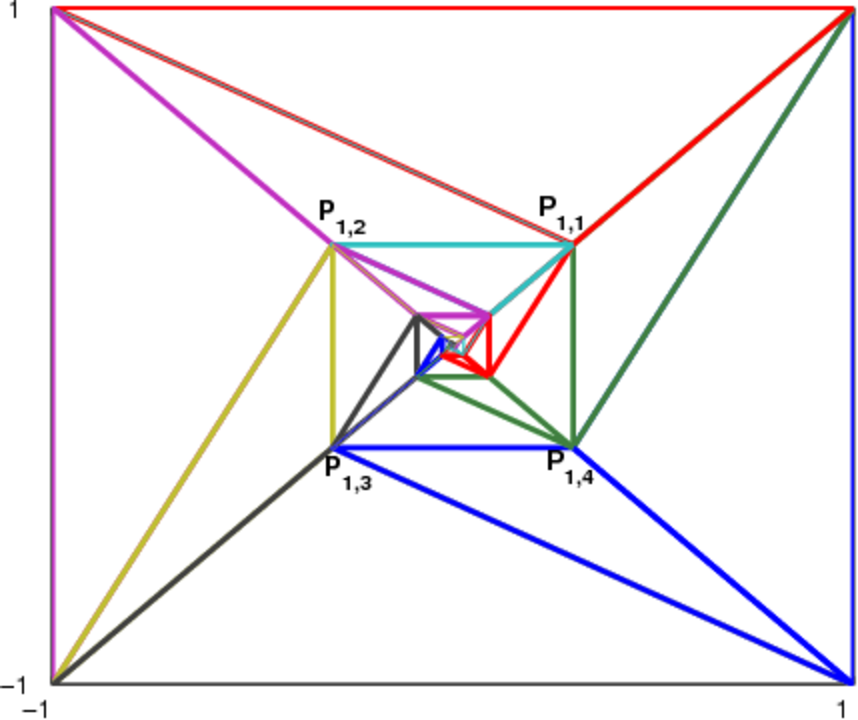
\includegraphics[width=\hsize]{Oswald/profOswald-fig1.png}
    \caption{Triangulation with large $L_\infty$ norm of the $L_2$-projector)}\label{fig:profOswald06}
   \end{center}
\end{figure}
The $L_\infty$-boundedness of
these projectors is of crucial importance for finite element error
estimates and the construction of orthogonal spline bases, and 
had been established for regular triangulations.
Our example shows for the first time that such regularity assumptions on the triangulations
are necessary. See \cite{Oswald2007a}, where also the higher-dimensional case
is negatively settled.

Polarization mode dispersion is a limiting factor for
operating long-haul optical fiber networks at high bitrates, and
its compensation is achieved by feedback-controlled
optical filters. As the result of joint work with
C.K. Madsen, we have published 
a fast and robust control algorithm for so-called
polarization controllers \cite{Oswald2006a}
which are used for a multitude of functions in an optical
fiber communication system. We currently explore the reuse 
of our control algorithms and architectures for other applications,
e.g.\ optical phase modulators. First contacts with the group
of Prof.~R. Noe (Uni Paderborn, EE Department)
led us to continuing with investigations into the theoretical
foundations of PMD theory, where there seems to emerge a new 
approach to higher order PMD characterization using uniform
approximations of the channel transfer matrix over the frequency band
of interest. 

This applied research is complemented by approximation-theoretic research
which backs up the observed improvement obtained from $N$-stage
filter architectures with increasing $N$ in a quantitative way.
After initial findings reported last year (M.Sc thesis by T. Shingel),
we have now proved a general bound for the approximation quality for
$SU(2)$-valued periodic transfer functions by $N$-stage finite impulse 
response (FIR) filters. The precise mathematical statement is as follows:
Any $SU(2)$-valued loop with finite $Lip_\alpha$ norm ($\alpha>1/2$) can be uniformly
approximated by an $N$-th degree polynomial loop with error $\le CN^{-\alpha/(1+\alpha)}$
as $N\to \infty$ (to be submitted soon). To the best of our knowledge, 
this is the first general result in another direction of
nonlinear approximation: polynomial approximation of functions with values in a
nonlinear manifold (in contrast to a linear space). Local approximation 
schemes for manifold-valued functions and data sets have attracted a lot of 
attention lately (e.g., in connection with symplectic integrators for Hamiltonian
ODEs, or in representing data attached to geometric objects), 
and we add another, even more classical angle to this.

\paragraph{Collaborations}
\begin{enumerate}
\item {\sl Texas A\&M University, USA} \\
Prof.~C.K. Madsen \\
Polarization control algorithms
\item {\sl Universi\"at Bonn, Germany} \\
Prof.~M. Griebel,  Dr.~M.-A. Schweitzer \\
Multilevel Algorithms for PDE
\item  {\sl CalTech, Pasadena, USA } \\
Prof.~P. Schr\"oder \\
Subdivision methods for 3D multiscale simulations
\end{enumerate}

